\documentclass{article}

\usepackage{caption}

\usepackage{multirow}

\usepackage[draft]{graphicx}
\setlength{\abovecaptionskip}{10pt plus 3pt minus 2pt}
\setlength{\belowcaptionskip}{10pt plus 3pt minus 2pt}

\usepackage[margin=1in]{geometry}

\usepackage{hyperref}
\hypersetup{
    pdfborderstyle={/S/U/W 1},
    colorlinks=true,
    linkcolor=blue,
    filecolor=magenta,
    urlcolor=cyan,
}

\usepackage{algorithm,algpseudocode}

\usepackage{xcolor}
\usepackage{listings}
\lstdefinestyle{DOS}{
    backgroundcolor=\color{lightgray},
    basicstyle=\scriptsize\color{black}\ttfamily
}

\title{\vspace{-2em}
CSE 5441 (Fall 2019, Dr. Jones)\\
\large \texttt{CUDA} (Lab 4)
}
\author{
Caleb Lehman \\
\href{mailto:lehman.346@osu.edu}{lehman.346@osu.edu}
}

\begin{document}
\maketitle

\section*{Overview}
\label{sec:overview}

For this lab, I modified my serial \texttt{C} program to perform Adaptive Mesh
Refinement (AMR)\footnote{See lab 1 or project descriptions for details about
AMR computation.} to work in parallel using the \texttt{CUDA} API. I created 2 programs,
\texttt{cuda-disposable} and \texttt{cuda-persistent}, which mirror the
disposable and persistent threads models used in the previous labs. In
particular, the \texttt{disposable} code runs a new kernel for each iteration,
while the \texttt{persistent} code has a single kernel which synchronizes the
threads between iterations\footnote{Because the \texttt{CUDA} API doesn't directly provide a simple way
to synchronize blocks, the \texttt{cuda-persistent} version is limited to running with a single block of
threads.}.

\section*{Tests}
\label{sec:tests}

\subsection*{Environment}
\label{subsec:environment}

The program was developed and tested on the
\href{https://www.osc.edu/resources/technical_support/supercomputers/owens}{Owens
cluster} at the \href{https://www.osc.edu/}{Ohio Supercomputer Center}.  Note
that all my other labs were developed and tested on the
\href{https://www.osc.edu/resources/technical_support/supercomputers/pitzer}{Pitzer
cluster}, which has different specs.

For development and testing, I loaded the \texttt{cuda/9.2.88} module, which
allowed the program to be compiled with version 9.2.88 of the \texttt{nvcc}
compiler, as well as setting some environment variables pointing to
\texttt{CUDA}-related headers and libraries.

For testing, I loaded the \texttt{python/3.6-conda5.2} module, which loads a
python environment with the \texttt{NumPy}, \texttt{SciPy}, and
\texttt{Matplotlib} packages, amoung others. \texttt{Python} is only necessary
for collecting and plotting the data from testing, not for the actual exectuion
of the program.

\subsection*{Timing}
\label{subsec:timing}

I collected timing data using the same 4 methods as the first lab:
\texttt{time}, \texttt{clock}, and \texttt{clock\textunderscore gettime} from
the \texttt{"time.h"} header, and the \texttt{UNIX} utility \texttt{time}.

As with the second and third labs, I didn't use the results from the \texttt{clock}
function from the \texttt{"time.h"} header, since it reports CPU time, not wall
time. The other methods all returned values within 1 second of each other. The
\texttt{time} function declared in \texttt{"time.h"} returns an integer number
of seconds, but the other two methods return with sub-second precision.
\emph{For consistency, I used the \texttt{clock\textunderscore gettime}
function for all results in this report}.

\subsection*{Test Files}
\label{subsec:test_files}

Dr. Jones provided the \texttt{testgrid\textunderscore 400\textunderscore
12206} test file.  As part of lab 1, I reduced the $\alpha$ (affect rate) and
$\varepsilon$ parameters until the serial runtime increased into the 3 to 6
minute range. In particular, I selected $\alpha = 0.01$ and $\varepsilon =
0.02$, for which the serial program completed in 261 seconds. However, my \texttt{CUDA}
implementations yielded very poor performance (more information in
\hyperref[sec:results]{Results} section), so I ended up using parameters of
$\alpha = 0.1$ and $\varepsilon = 0.1$.  For this reason, and due to using the
Owens cluster instead of the Pitzer cluster, it isn't particularly useful to
compare the results from this lab to the results from labs 2 and 3.

\newpage
\section*{Results}
\label{sec:results}

The output was consistent across both programs and was as follows:
\begin{itemize}
    \item \texttt{testgrid\textunderscore 400\textunderscore 12206}: 1589637 iterations, $(max, min) = (0.085900, 0.084182)$
\end{itemize}

The relevant runtimes for the serial, \texttt{cuda-persistent}, and \texttt{cuda-disposable}
versions on the test case can be found below.

\textbf{TODO} Best parameters. Really poor performance, unsure why.
Potentially due to very short iterations.

\textbf{TODO} With comparable parameters, \texttt{cuda-disposable} as good (better) than \texttt{cuda-persistent},
confirming very light-weight threads.

\textbf{TODO} GFlops.

\vspace{1em}
\begin{minipage}{\linewidth}
    \centering
    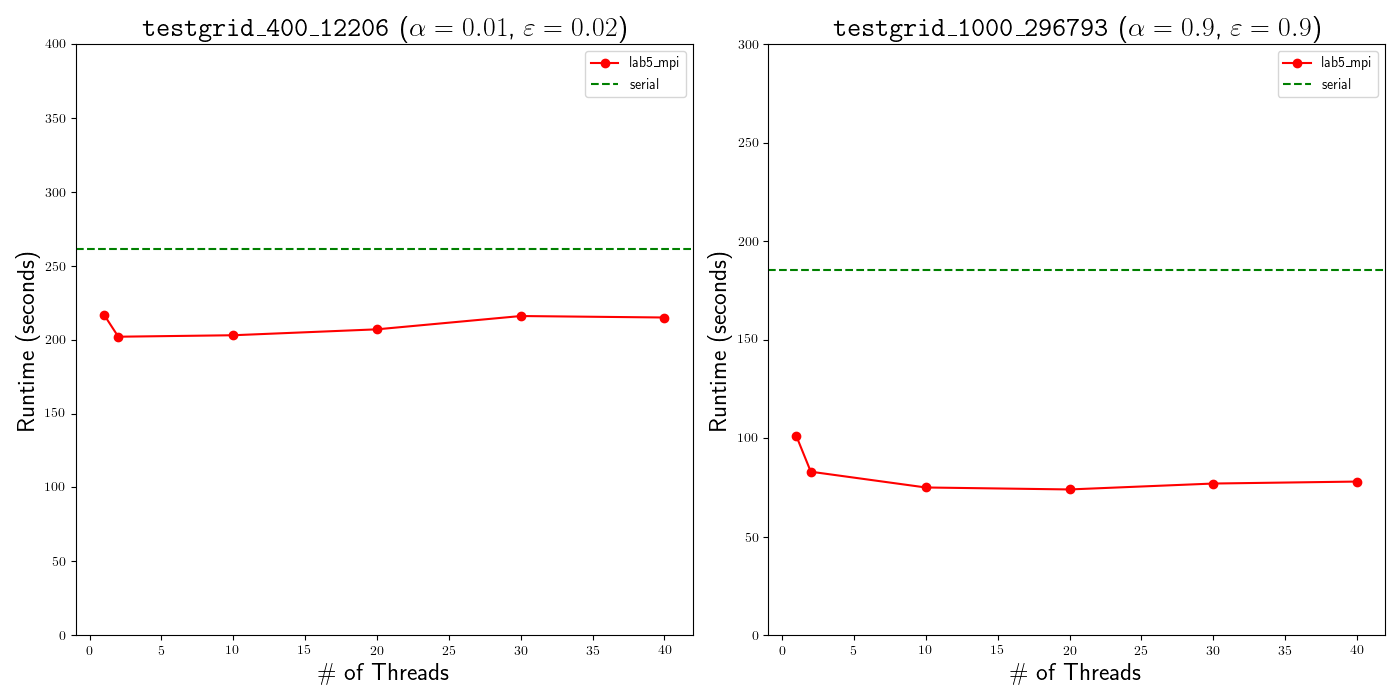
\includegraphics[width=.8\linewidth]{../results/plot.png}

    \captionof{figure}{The runtimes of the parallel versions (\texttt{pthreads}
    and \texttt{OpenMP}) of the program plotted against the number of threads
    used. Serial runtime is included for comparison. Note that \texttt{OpenMP}
    \texttt{persistent} and \texttt{disposable} versions consistently perform
    nearly identically.}

    \label{fig:runtimes}
\end{minipage}

\section*{Project Usage}
\label{sec:project}

\subsection*{Building}
\label{subsec:building}

To build the \texttt{cude-disposable} and \texttt{cude-persistent} executables, navigate
to the top level of the submitted directory and build as follows:

\begin{lstlisting}[style=DOS]
# Ensure that you have nvcc compiler

# Note that the provided makefile
# assumes the CUDA_HOME environment
# variable is set appropriately

# On the OSC clusters, this can be achieved
# with the command:
$ module load cuda

$ make
$ ls
... cuda-persistent cuda-disposable ...
\end{lstlisting}

\subsection*{Running}
\label{subsec:running}

The syntax to run the program is:

\begin{lstlisting}[style=DOS]
$ ./[program] [affect-rate] [epsilon] <[test-file]
\end{lstlisting}
where \texttt{program} is one of $\{\texttt{cuda-persistent}, \texttt{cuda-disposable}\}$

\end{document}
